%
% Norbert Preining
% Article presented on the 5th GuITmeeting, Pisa 18 October 2008
%
% Copyright 2008 Norbert Preining
% You can redistribute and/or modify this document under the terms of the 
% GNU General Public License as published by the Free Software Foundation; 
% either version 2 of the License, or (at your option) any later version.
%
\documentclass{arstexnica}
\usepackage[utf8]{inputenc}
\usepackage[T1]{fontenc}
\usepackage{lmodern}
\usepackage[english]{babel}
\usepackage{graphicx}
\usepackage{hyperref}
\usepackage{fancyvrb}
\usepackage{url}
\usepackage{natbib}
\usepackage{marvosym}
\usepackage{listings}
\lstset{frame=lines,basicstyle=\small\ttfamily,prebreak={\Righttorque},
        postbreak={\Lefttorque},columns=flexible}%,breaklines}
\newcommand{\tl}{\TeX~Live}
\newcommand{\tlmgr}{\TeX~Live Manager}

\newcommand{\tlpsrc}{\texttt{tlpsrc}}
\newcommand{\tlpsrcs}{\tlpsrc{}s}
\newcommand{\tlpobj}{\texttt{tlpobj}}
\newcommand{\tlpobjs}{\tlpobj{}s}
\newcommand{\tlpdb}{\texttt{tlpdb}}
\newcommand{\tlpdbs}{\tlpdb{}s}
\newcommand{\pl}{Perl}
\newcommand{\gs}{Ghostscript}
\newcommand{\tlu}{\texttt{texlua}}
\newcommand{\kpse}{Kpathsea}
\newcommand{\XeTeX}{Xe\TeX}
\newcommand{\acro}[1]{\textsc{\MakeLowercase{#1}}}
\newcommand{\ctan}{\acro{CTAN}}
\newcommand{\cmd}[1]{\textsf{#1}}
\newcommand{\button}[1]{\textsf{#1}}
\newcommand{\var}[1]{\textsl{#1}}

\hyphenation{infra-struc-ture}

%\catcode`>=\active
%\def>#1<{\texttt{#1}}
\DefineShortVerb{\|}
\begin{document}
\begin{article}
%\selectlanguage{italian}%

\title{\tl~2008 and the \TeX\ Live Manager%
  \thanks{Originally presented at the \GuIT\ Conference 2008 in Pisa, and
          published in Ars\TeX nica, issue~6}}

\author{Norbert Preining}
\address{Vienna University of Technology\\
	%Wiedner Hauptstr.\ 10\\
	%1040 Wien, Austria
}
\netaddress{preining@logic.at}

\maketitle


\begin{abstract}
\tl~2008 has been released recently, and the \acro{DVD}s are ready to
go gold. This is the first release of \tl\ shipping the \tlmgr, tlmgr 
for short.

Besides taking over some of the tasks from texconfig (which has never been
available for Windows) it finally brings many new features
to the \tl\ world, most importantly the option for dynamic updates.

This article will present the new \tl\ Installer, the \tlmgr, and
at the end lists other changes in \tl~2008.
\end{abstract}

\tableofcontents

\section*{Important note}

This article describes the status of the \tlmgr\ as it will be shipped
around October~2008, and not the one on \acro{DVD}. The
version on the \acro{DVD} works fine for local configuration
tasks (which is why we felt it could be shipped), but is not
sufficiently robust for reliable updates over the Internet.  Users'
first update will be to get the new tlmgr.

\section{Introduction}
\label{sec:intro}

After more than one year of development work \tl~2008 has been
released with a complete new infrastructure \citep{at:2007-4-069-preining}.
At first these infrastructure changes were only relevant for the
developers themselves, since it made life (a bit) easier and the
system more consistent due to the elimination of duplicated
information. 

As a first user-visible change came the unification of the installer,
so that all supported platforms now share the same
installer. Furthermore, this installer has gotten a \acro{GUI} which
also is uniform across all platforms. On Unix systems the only
prerequsites are a Perl installation, and for the \acro{GUI} the
installation of Perl/Tk. On Windows we ship a minimal Perl with
the necessary modules.

The first part of this article will give an overview of the new
installer.

The second user-visible change came from the addition of the \tlmgr,
or tlmgr for short, to the list of programs. It manages an existing \tl\
installation, both packages and options. Besides performing  many of
the same actions as |texconfig| it has the ability to install 
additional packages, update and remove existing ones, make backups,
search within and list all packages.

\section{The new installer}
\label{sec:installer}

The creation of a new \tl\ installer was necessitated by the new
package infrastructure \citep{at:2007-4-069-preining}. From a user's
point of view the new installer has only one visual change, but there
other significant changes. In particular: 
\begin{itemize}
\item It is possible to install \tl\ from the Internet.
\item There is just one installer, which can run either in text
  mode, emulating the former install-tl.sh shell script,
  or in \acro{GUI} mode (more or less emulating the \tl\ 2007 tlpmgui).
\item The Windows installation is much closer to using the same
  implementation as Unix.
\end{itemize}

\subsection{Install \tl\ from the Internet}

If you got (by the time you read this article) a \tl\ \acro{DVD} you
can just start the installer as usual. On Windows this will be by
default the \acro{GUI} installer (see below), on Unix the text mode
installer. 

We also ship an installation package \citep{inst:package} containing
all the necessary files for an installation over the network. By
default, normal installation will use a \ctan\ mirror, 
selected using the |http://mirror.ctan.org| service.  (See
|http://tug.org/ctan.html#sites|.)

Two installers for network downloads are provided.
|install-tl-unx.tar.gz| supports Unix only.  |install-tl.zip|
additionally contains a small subset of Perl for Windows which is
required to bootstrap the system.  The latter works on all platforms
supported by \tl.  The sole reason for providing a separate package
for Unix is its significantly smaller size.

In any case you can override the source from which you want to install
with the command line option |-location|.

\subsection{The text mode installer}

If you have used \tl\ in recent years you will see no big changes in
the text mode installer (see fig.~\ref{fig:text_main_menu}); we tried
to keep it as close as possible to the one used in former
releases. One new option is at the bottom of the menu, namely
\emph{set up for running from DVD}. This is what we call \emph{live}
installation:
it sets up a minimal writable environment on your computer, while all the input
files and binaries remain on the \acro{DVD}. 

\begin{figure}[ht!]
  \centering
  \resizebox{\columnwidth}{!}{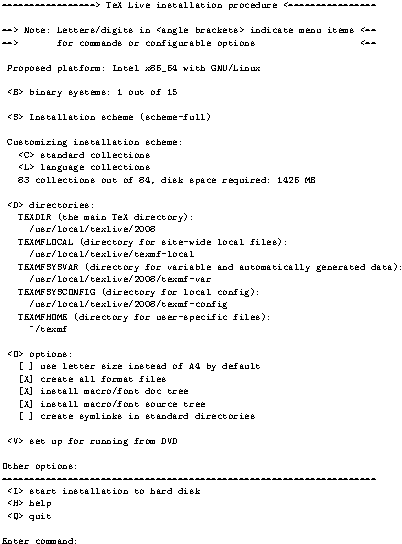
\includegraphics{install08text-crop}}
  \caption{Main menu of the text mode installer}
  \label{fig:text_main_menu}
\end{figure}

\subsection{The GUI Installer}

The \acro{GUI} installer has nearly the same functionality as the text
version; the option to set up for live installation is the only missing
piece. It is written in Perl/Tk and thus should run on all platforms (on
Unix Perl/Tk has to be installed).

\begin{figure}[ht!]
  \centering
  \resizebox{\columnwidth}{!}{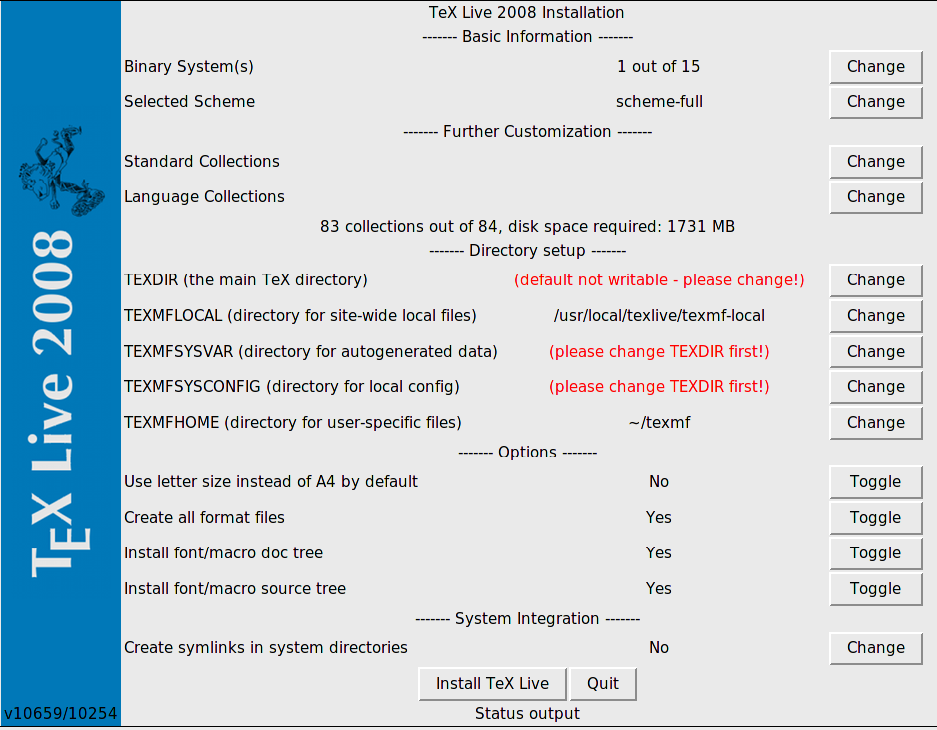
\includegraphics{gui-installer.png}}
  \caption{Main window of the \acro{GUI} installer}
  \label{fig:gui_main_menu}
\end{figure}

The main window can be seen in fig.~\ref{fig:gui_main_menu}. It should
remind you very much of the text mode installer. As with the text mode
installer it allows you to change which binary systems should be
installed (fig.~\ref{fig:gui_systems}), select the scheme to be
installed (fig.~\ref{fig:gui_scheme}), where a \emph{scheme} is a
pre-defined set of
collections to be installed, and further specify in more detail which
collections (a collection is a set of packages) and which language
packages to
install (fig.~\ref{fig:gui_coll} and~\ref{fig:gui_lang}). You
can select the installation directories for \tl\ and toggle some
options, all in line with the installer of recent years and the text
mode installer.

\begin{figure}[ht!]
  \centering
  \resizebox{0.5\columnwidth}{!}{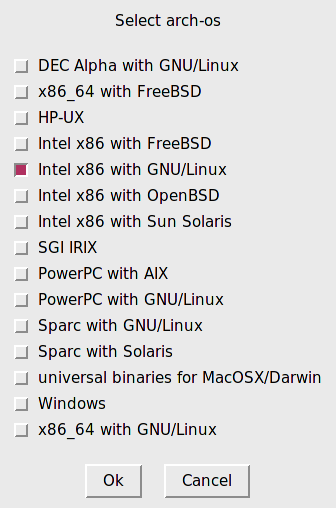
\includegraphics{gui-systems.png}}
  \caption{Binary system select window}
  \label{fig:gui_systems}
\end{figure}

\begin{figure}[ht!]
  \centering
  \resizebox{\columnwidth}{!}{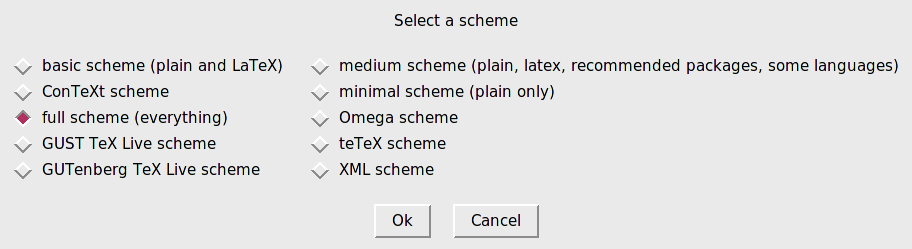
\includegraphics{gui-scheme.png}}
  \caption{Scheme select window}
  \label{fig:gui_scheme}
\end{figure}

\begin{figure}[ht!]
  \centering
  \resizebox{\columnwidth}{!}{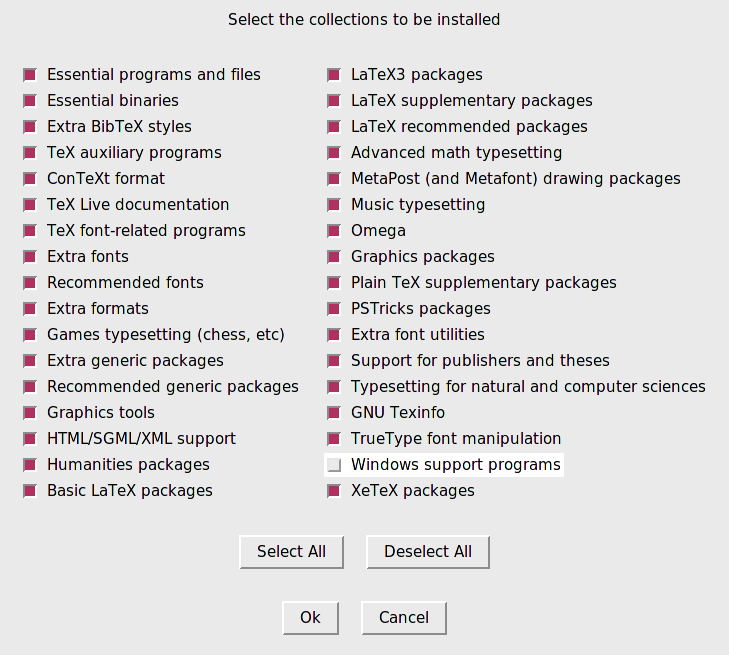
\includegraphics{gui-collections.png}}
  \caption{Collections select window}
  \label{fig:gui_coll}
\end{figure}

\begin{figure}[ht!]
  \centering
  \resizebox{\columnwidth}{!}{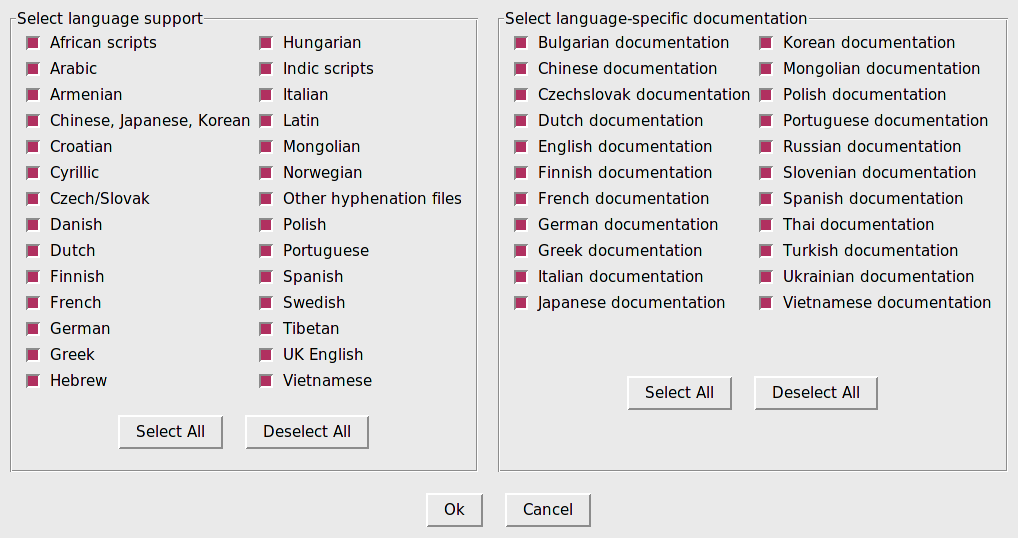
\includegraphics{gui-lang.png}}
  \caption{Language packs select window}
  \label{fig:gui_lang}
\end{figure}

During installation the main window's status line will indicate what
is going on currently, and at the same time the program will print out
to the terminal the same output as the normal installer.

For both the text mode installer and the \acro{GUI} mode installer, a
log file with more details is
created in the installation directory as |install-tl.log|. (If you
report installation problems, please send us this log file.)

\subsection{Bringing Windows in line with Unix}

\tl\ 2008 supports Windows 2000 and later. By dropping older Windows
versions, there is much less need to treat Windows specially.

Under Windows 2000 and later, users have a real home directory,
viz. \verb+%USERPROFILE%+, usually
\verb+C:\Documents and Settings\+\textit{username}.

This is now reflected in tilde expansion by \kpse:
\verb+~/texmf+ is expanded to \verb+%USERPROFILE%\texmf+
under Windows and to \verb+$HOME/texmf+ under Unix.

It is also possible to differentiate between system settings and
user settings. Happily, there is no longer any need to have a different
set of \texttt{texmf} trees on Windows, or to leave out scripts such as
\texttt{fmtutil-sys} and \texttt{updmap-sys}.  We also 
have a single \texttt{texmf.cnf} used on all platforms.


%
%
%
\section{The \tlmgr}

\tlmgr\ provides a wealth of options and commands; we will explain them
all here, some tersely, some in more detail.  Of course we expect to add
more features in the future.

\subsection{The \tl\ Database}

First of all, it is important to understand where all the information about
installed packages and other options are saved. This is the \tl\
database, which normally can be found in \path{ROOT/tlpkg/texlive.tlpdb}
(where |ROOT| is the destination folder you have choosen at
installation time). It contains the list of all packages, all the
files installed, and in addition to that collects configuration
information like the default installation source, and the options you
have set at installation time (e.g., whether you want A4 or letter-size
paper by default).

Most of tlmgr's actions will load the local database, and many
actions will also load a remote database: If you want to install a
package, the \tlmgr\ will load the database of the specified installation server
and checks whether this package exists. 

Although we say \emph{remote}, it is not necessarily a remote
network location. If you install from \acro{DVD} the default
installation source will be the \acro{DVD}, and tlmgr will 
load the database located on the \acro{DVD} when needed.

\subsection{General syntax of tlmgr}

The general syntax of tlmgr is
\begin{center}
  \Verb+tlmgr [opt]... action [opt]... [arg]...+
\end{center}
The first set of options before the main |action| configure the general
operation of tlmgr, while the second set of options are specific to
the chosen |action|. We do not support mixing and reshuffling of all
these options, partly for the sake of clarity, and also for programming
reasons. 

The first set of options can contain
\begin{itemize}
\item |--location| \var{loc} specifies the location from which
  packages should be installed or updated, overriding the location
  found in the installation's \tl\ Package Database (\acro{TLPDB}).
\item |--gui| starts the \acro{GUI} version of tlmgr.
  The \acro{GUI} does not support all the bells
  and whistles of the command-line program. It is in fact a separate
  program that calls the command-line version to do the actual work.
  The difference between this |--gui| option and the |gui| action (see
  below) is that given the option,
  tlmgr tries to open the \acro{GUI} directly at the screen
  for the specified |action|.
\item |--gui-lang| \var{ll} selects the language in which the \acro{GUI} will
  appear. Normally the \acro{GUI} tries to deduce your language from
  the environment (on Windows via the registry, on Unix via
  |LC_MESSAGES|). If that fails you can select a different language by
  giving this option a two-letter language code.
\end{itemize}

Furthermore, some standard options are supported: |--help| (also |-h|)
for getting help, |-q| which supresses informational messages, and
|-v| (verbose) for turning on debugging options. With |--version| the
script will show you the version of your \tl\ system and of itself. 

\subsection{The actions}

There is a (permanently growing) list of actions, currently: |help|, |version|,
|gui|, |install|, |update|, |backup|, |restore|, |remove|, |option|,
|paper|, |arch|, |search|, |show|, |list|, |check|, |uninstall|, |generate|.

\paragraph{The general actions}

\begin{itemize}
\item |search [|\var{option}|...] |\var{what} Without any options, search in the list
  of locally installed packages for package names or descriptions
  matching |what|. If you give the option |--global| it also searches
  the remote database. This might differ in case you have not
  installed all of \tl, but only a part of it. Finally, if you specify
  |--file| then files are searched, and not package names.
\item |show |\var{pkg}|...| gives you more detailed information on the
  listed packages. If all packages are installed locally, it does not
  consult the remote database.
\item \Verb+list [collections|schemes]+ With no argument, lists all
  packages available at the default install location, prefixing those
  already installed with "i ". With an argument lists only collections
  or schemes, as requested. 
\item |uninstall| This action will ask for confirmation, and then remove
  the entire installation. Don't do it or we will be sad. If you give
  the |--force| option, it does not even ask, but proceeds
  immediately with the removal.
\item \Verb+check [files|collections|all]+ Executes one (or all)
  check(s) on the consistency of the installation. For |files| it
  checks that all files listed in the local database
  are actually present, and lists those missing.%
%  \footnote{On Windows that will not work currently, since
%    Windows does not ship find. Also MacOS seems to ship a strange
%    find implementation that does not support -wholename, so that
%    will break, too.}
  The option |--use-svn| will use the |svn| command to check for the
  files. 
\item |gui| starts the \acro{GUI}, as explained above at |--gui|.
\item |version| is the same as |--version|.
\item |help| is the same as |--help|.
\end{itemize}

\paragraph{The configuration actions}
\begin{itemize}
\item |option [show]| Shows all configuration settings currently
  saved in the local database.  The |show| option is accepted and ignored.
\item |option |\var{key} |[|\var{value}|]| Without the
  \var{value}, shows the current value
  of the configuration option \var{key}; with \var{value}, sets this
  configuration option. Currently accepted |key|s are |location|
  (default installation location), |formats| (create formats at
  installation time), |docfiles| (install documentation files),
  |srcfiles| (install source files). These are the options you have
  set at installation time and will be honoured at \emph{later} install and
  upgrade actions.  For example, changing the |docfiles|
    options from false to true will not install or remove the already
    present documentation files. But a subsequent update will install or remove
    them.
\item |paper |\var{paper} Sets the default papersize; possible values
  are |a4| and |letter|.
\item \var{program} \Verb+paper [help|+\var{paper}|]|
  This allows setting different paper sizes for the specified
  \var{program}: |xdvi|, |dvips|, |pdftex|, |dvipdfm|,
  |dvipdfmx|, |context|. Without any additional argument it reports the 
  currently selected papersize. With |help|, it issues all the
  supported paper sizes for that program. And if you specify a paper size,
  it will be set as default papersize for the given program.
\item |generate |\var{what} This command generates one or more 
  configuration files, as follows:
  
  Giving |language.dat| for \var{what} 
  generates the |language.dat| file which specifies the
  hyphenation patterns to be loaded for \LaTeX-based formats.
  Giving |language.def| for \var{what} generates the |language.def|
  file which specifies hyphenation patterns to be loaded for
  |etex|-based formats.
  Specifying |language| for |what| 
  generates both of these files.
  
  Giving |fmtutil| for \var{what} generates the |fmtutil.cnf| file which
  contains the definitions of all formats available.

  Giving |updmap| for \var{what} generates the |updmap.cfg| file which
  lists all the installed font map files.

  For |fmtutil| and the language files, recreating is normal and both the
  installer and tlmgr routinely call that.

  For |updmap|, however, neither the installer nor tlmgr use
  |generate|, because the result would be to disable all maps which
  have been manually installed via |updmap-sys --enable|, e.g., for
  proprietary or local fonts.  Only the changes in the |--localcfg|
  file mentioned below are incorporated by |generate|.

  On the other hand, if you only use the fonts and font packages
  within \TeX\ Live, there is nothing wrong with using |generate updmap|.
  Indeed, we use it to generate the |updmap.cfg| file that is
  maintained in the live source repository.

  If the files |language-local.dat|, |language-local.def|,
  |fmtutil-local.cnf|, or |updmap-local.cfg| are present under
  \path{TEXMFLOCAL} in the respective directories, their contents will
  be simply merged into the final files, with no error checking of any
  kind. 
\end{itemize}


\paragraph{The package management actions}
\begin{itemize}
\item |install| \var{pkg}\ldots\ installs the packages given as argument. 
  By default, installing a package
  also installs all of its dependencies. 
  The following options are supported: |--no-depends| will
  not install dependent packages. There is also |--no-depends-at-all|
  which in addition
  disregards the tightly coupled packages architecture-specific
  executables; for example,
  |bin-bibtex| and |bin-bibtex.i386-linux|. That is something you
  should never use unless you are sure you know what you are
  doing. |--dry-run| fakes the installation without changing anything.
\item |update| \var{pkg}\ldots\  updates the packages given as arguments. 
  In addition, if the \var{pkg} is a collection, and the remote server
  has new packages in this collection, they will be installed,
  following the dependencies specified in the collection.  Options:
  \begin{description}
  \item |--list| Lists the packages which would be updated or newly
    installed, but does not do the update. It also lists the revision
    numbers of the local and the remote packages.
  \item |--all| Update all out-of-date packages.
  \item |--dry-run| Fake the updates without changing anything.
  \item |--backupdir |\var{directory}
    Save a snapshot of the current package (as installed) in \var{directory},
    before the package is updated. This way one can easily recover
    in case an update turned out as not working. See the 
    |restore| action for details.
  \item |--no-depends| Do not install normal dependencies.
  \item |--no-depends-at-all| See |install| above for this option.
  \end{description}
\item |remove| \var{pkg}\ldots\ 
  removes the packages given as arguments.  Removing a
  collection will remove all package dependencies (but not collection 
  dependencies) in that collection, unless |--no-depends| is
  specified.  However, when removing a package, dependencies are
  never removed.

  Options:
  \begin{description}
  \item |--no-depends| Do not remove dependent packages.
  \item |--no-depends-at-all| See |install| above for this option.
  \item |--force|
    By default, when removing a package or collection would
    invalidate a dependency of another collection/scheme, the
    package is not be removed and an error is given.  With this
    option, the package will be removed unconditionally.  Use with
    care.
  \item |--dry-run|
    Fake the removals without actually changing anything.
  \end{description}
\item |backup| \var{pkg}\ldots\
  makes a backup of the given packages, or all packages
  with |--all|, to the directory specified with |--backupdir| (must
  exist and be writable.

  The following options are supported:
  \begin{description}
  \item |--backupdir |\var{directory}
    The directory is a required argument and must specify an existing
    directory where backups are to be placed.
  \item |--all|
    Make a backup of all packages in the \TeX\ Live installation.
    This will take quite a lot of space and time.
  \end{description}

\item |restore --backupdir |\var{dir} |[|\var{pkg} |[|\var{rev}|]]|\\
  If no |pkg| is given (and thus no |rev|), lists the available backup
  revisions for all packages.
 
  With |pkg| given but no |rev|, list all available backup revisions
  of |pkg|.

  With both |pkg| and |rev|, tries to restore the package from the
  specified backup.

  The option |--backupdir dir| is required, and must specify a
  directory with backups.
  
  The option |--dry-run| is also supported, as usual.
  
\item |arch |\var{operation} \var{arg}\ldots
  If \var{operation} is |list|, this
  lists the names of architectures (|i386-linux|, \ldots)\ available at
  the default install location.
  
  If \var{operation} is |add|, adds the executables for each of the following
  arguments (architecture names) to the installation.
  
  The option |--dry-run| is also supported, as usual.
\end{itemize}


\subsection{Typical usage of tlmgr}

Here we present some typical usage examples of the \tlmgr.

\paragraph{Installing a new collection}

Suppose that you installed |scheme-medium| and then realize that the
hyphenation patterns for some language you are using haven't been
installed, say, Norwegian. First you fire up tlmgr to search for
the support: 
\begin{lstlisting}
$ tlmgr search --global norwegian
collection-langnorwegian - Norwegian
hyphen-norwegian - 
\end{lstlisting}
and then to install this collection:
\begin{lstlisting}
$ tlmgr install collection-langnorwegian
install: collection-langnorwegian
install: hyphen-norwegian
regenerating language.dat
regenerating language.def
\end{lstlisting}
and then it continues to regenerate all the format files depending on
either |language.dat| or |language.def|. (If the
the |formats| option is changed to false in the local database, the
format rebuilding will be skipped.  The default is to do so, to keep
them up to date without manual intervention.)


\paragraph{Searching for a package}

You want to typeset an invitation in a special form, say 
in the shape of a heart. Your first try is
\begin{lstlisting}
$ tlmgr search paragraph
\end{lstlisting}
but that yields no output. Maybe it's not installed?
So try a global search:
\lstset{breaklines}
\begin{lstlisting}
$ tlmgr search -global paragraph
tlmgr: installation location /src/TeX/texlive-svn/Master
 bigfoot - Footnotes for critical editions
 edmargin - Multiple series of endnotes for critical editions
 footmisc - A range of footnote options
 genmpage - Generalization of LaTeX's minipages
 hanging - Hanging paragraphs
 ibycus-babel - Use the Ibycus 4 Greek font with Babel
 insbox - A TeX macro for inserting pictures/boxes into paragraphs
 layouts - Display various elements of a document's layout
 lettrine - Typeset dropped capitals
 lineno - Line numbers on paragraphs
 lipsum - Easy access to the Lorem Ipsum dummy text
 moresize - Allows font sizes up to 35.83pt
 ncctools - A collection of general packages for LaTeX
 paralist - Enumerate and itemize within paragraphs
 picinpar - Insert pictures into paragraphs
 plari - Typesetting stageplay scripts
 seqsplit - Split long sequences of characters in a neutral way
 shapepar - A macro to typeset paragraphs in specific shapes
 vwcol - Variable-width multiple text columns
\end{lstlisting}
and here we are, \texttt{shapepar} seems to be what's needed. So let
us see what it is:
\begin{lstlisting}
$ tlmgr show shapepar
tlmgr: installation location /src/TeX/texlive-svn/Master
Package:   shapepar
Category:  Package
ShortDesc: A macro to typeset paragraphs in specific shapes.
LongDesc:  \shapepar is a macro to typeset paragraphs in a
special ...
Installed: No
Collection:collection-latexextra
\end{lstlisting}
Ok, confirmed, now we can either install the
respective collection using
\begin{lstlisting}
$ tlmgr install collection-latexextra
\end{lstlisting}
which will install quite a lot of packages, or only that one single
package in the hope that it does not depend on anything else:
\begin{lstlisting}
$ tlmgr install shapepar
tlmgr: installation location /src/TeX/texlive-svn/Master
install: shapepar
running mktexlsr
...
\end{lstlisting}

These examples are about finding uninstalled packages.  The default for
\tl\ is a full installation, i.e., everything is installed that is
available.

\paragraph{Updating your installation}

After the initial installation you want to get the latest and
greatest of everything, but first you want to see what that means:
\begin{lstlisting}
$ tlmgr update --list
tlmgr: installation location /mnt/cdrom
Cannot load TeX Live database from /mnt/cdrom at /home/norbert/tltest/2008/bin/i386-linux/tlmgr line 1505, <TMP> line 1982.
\end{lstlisting}
Hmm, there seems to be an error, it tries to install from the \acro{DVD}
which you returned to your friend last week. Well, then you
should switch to the network installation source; best to do it
for all future sessions by saving it as default
location. But what was that strange address again? Fortunately you can
tell tlmgr to use \acro{CTAN} and it will know what to do:
\begin{lstlisting}
$ tlmgr option location ctan
tlmgr: setting default installation location to http://mirror.ctan.org/systems/texlive/tlnet/2008
\end{lstlisting}
Fine. Now let us see what we can upgrade:
\begin{lstlisting}
$ tlmgr update --list
shapepar: local: 10400, source: 10567
bin-texlive: local: 10693, source: 10750
pdftex: local: 10622, source: 10705
texlive.infra: local: 10685, source: 10748
\end{lstlisting}
Well, some things are there, so let us update all of them at once:
\begin{lstlisting}
$ tlmgr update --all
update: shapepar (10400 -> 10567) ... done
update: bin-texlive (10693 -> 10750) ... done
update: pdftex (10622 -> 10705) ... done
update: texlive.infra (10685 -> 10748) ... done
running mktexlsr ...
\end{lstlisting}

\paragraph{Paper size configuration}

You are moving to Japan and want letter as your default paper size;
nothing easier:
\begin{lstlisting}
$ tlmgr paper letter
\end{lstlisting}
will switch to letter for the most important programs, and at also
recreate the formats.

\section{The GUI for tlmgr}

To make most Windows users and some Unix users happy we provide a
front end for the \tlmgr\ written in Perl/Tk. It does not do the
actual work, but leaves that for tlmgr.  It also does not provide quite the
full functionality of tlmgr, but almost all of it is there.

This program features several screens for different functionalities:
installation, update, and removal of packages, removal of \tl\ as a
whole, architecture support and configuration.

The \acro{GUI} is started with either \texttt{tlmgr gui} or
\texttt{tlmgr --gui action} where \texttt{action} is one of the
actions given above. In the latter case it tries to open the respective screen of
the \acro{GUI}.

\subsection{The install screen}

The first window to be seen normally is the package installation
screen (fig.~\ref{fig:gui:install}).

\begin{figure}[ht!]
  \centering
  \resizebox{\columnwidth}{!}{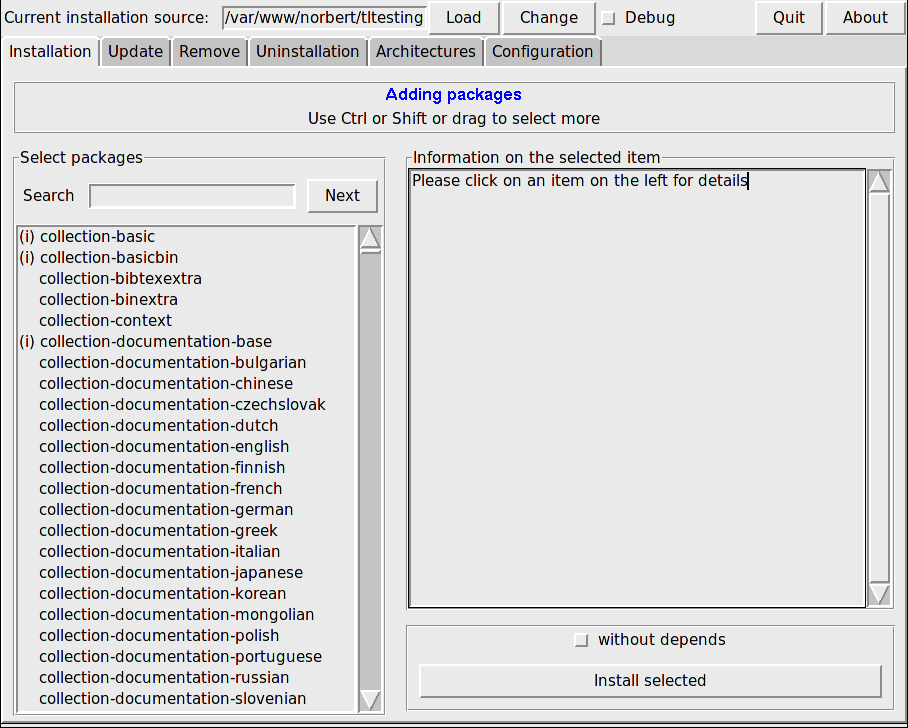
\includegraphics{tlmgrgui-install.png}}
  \caption{\tlmgr\ \acro{GUI} install screen}
  \label{fig:gui:install}
\end{figure}

At the top you see the current installation source, as given either on
the command line of tlmgr, or in the absence of a command line
argument as taken from the default option. It is \emph{not} loaded
automatically, you have to press the \button{Load} button, or the
\button{Change} button to select a different installation source for
this run only. Below you see the list of available packages on the
left, first all the collections and schemes, then all the
other packages in alphabetic order. You can search by entering a
string into the search text field, which immediately jumps to the
first entry. The button \button{Next} jumps to the next match. After
selecting one package you can see its description in the right half of
this screen. Below there is the action button for installing the
selected package(s), and also a switch that allows you to install a
package without those it depends on.

\subsection{The update screen}

The update screen is similar to the install screen, but only
lists those packages which have an upgrade available on the
installation location. The upper part of the right pane gives you
information on the package, and in the action area below you see two
buttons, one for updating only the selected packages, and one for
updating all packages.

In fig.~\ref{fig:gui:update} you can see the update screen with
updates available and the information for the selected package shown
in the right part of the screen. 

\begin{figure}[ht!]
  \centering
  \resizebox{\columnwidth}{!}{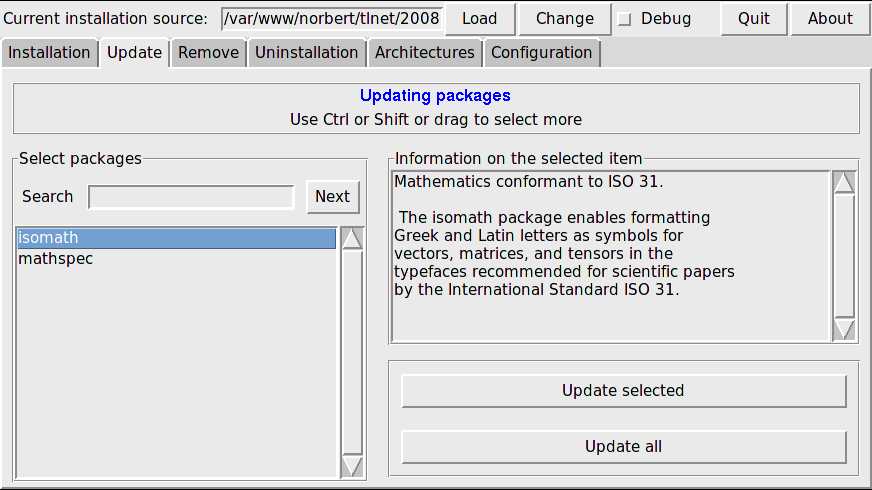
\includegraphics{tlmgrgui-update.png}}
  \caption{\tlmgr\ \acro{GUI} update screen}
  \label{fig:gui:update}
\end{figure}

\subsection{The remove screen}

The remove screen is also similar to the install screen, with the
list of all installed packages in the left part, the
information window in the upper right part, and the action area with
two toggles and the remove button in the lower right part; see
fig.~\ref{fig:gui:remove}.

The two toggles correspond to the option |--force| and |--no-depends|
of the tlmgr |remove| action, see above.

\begin{figure}[ht!]
  \centering
  \resizebox{\columnwidth}{!}{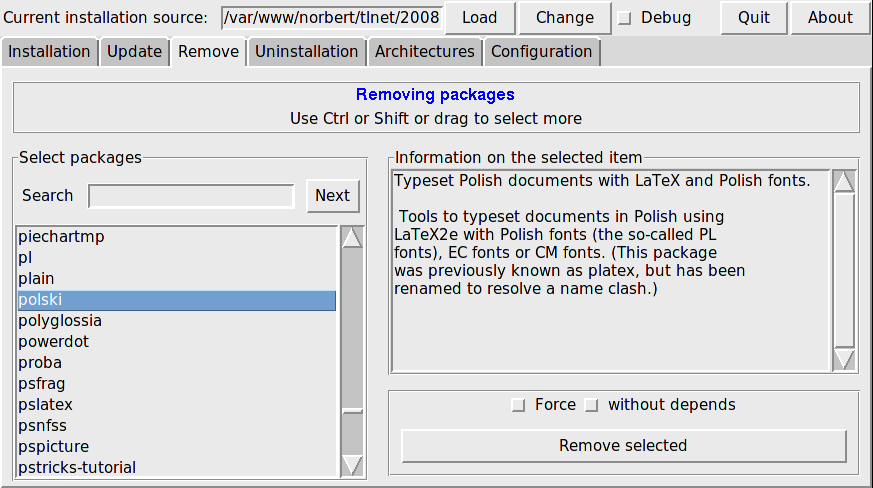
\includegraphics{tlmgrgui-remove.png}}
  \caption{\tlmgr\ \acro{GUI} remove screen}
  \label{fig:gui:remove}
\end{figure}

\subsection{The uninstallation screen}

This screen only sports one button which allows you to completely remove
the \tl\ installation from your system. This button is not present on
Windows systems, being replaced by an informational note that you should
use the \cmd{Add/Remove} entry from the Control Panel.

\subsection{The architectures screen}

\tl\ allows you to install the binaries for several
architecture-operating system combinations in case you want to
distribute your installation via \acro{NFS} or other means in an
inhomogen local network, see fig.~\ref{fig:gui:arch}.

\begin{figure}[ht!]
  \centering
  \resizebox{\columnwidth}{!}{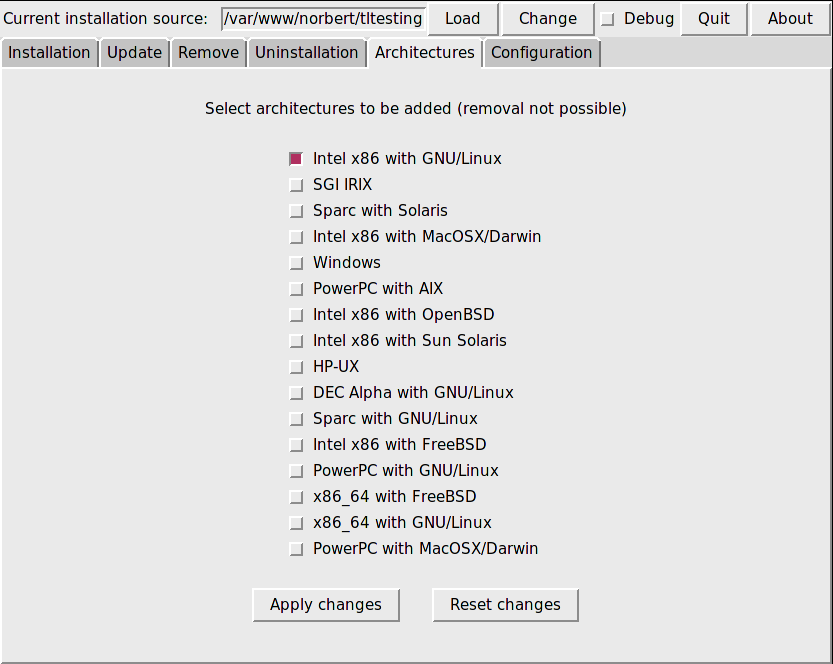
\includegraphics{tlmgrgui-arch.png}}
  \caption{\tlmgr\ \acro{GUI} architectures screen}
  \label{fig:gui:arch}
\end{figure}

This screen lists the available architectures at the current
installation source, and allows you to select new architectures to be
installed by pressing the \button{Apply changes} button.

Note that the \emph{removal} of architectures is currently not
supported, and that the whole screen is disabled on Windows systems
since Windows does not support normal symbolic links.

\subsection{The config screen}

This screen allows the user to comfortably examine and set the various
options of the \tl\ installation, see figure~\ref{fig:gui:option}.

\begin{figure}[ht!]
  \centering
  \resizebox{\columnwidth}{!}{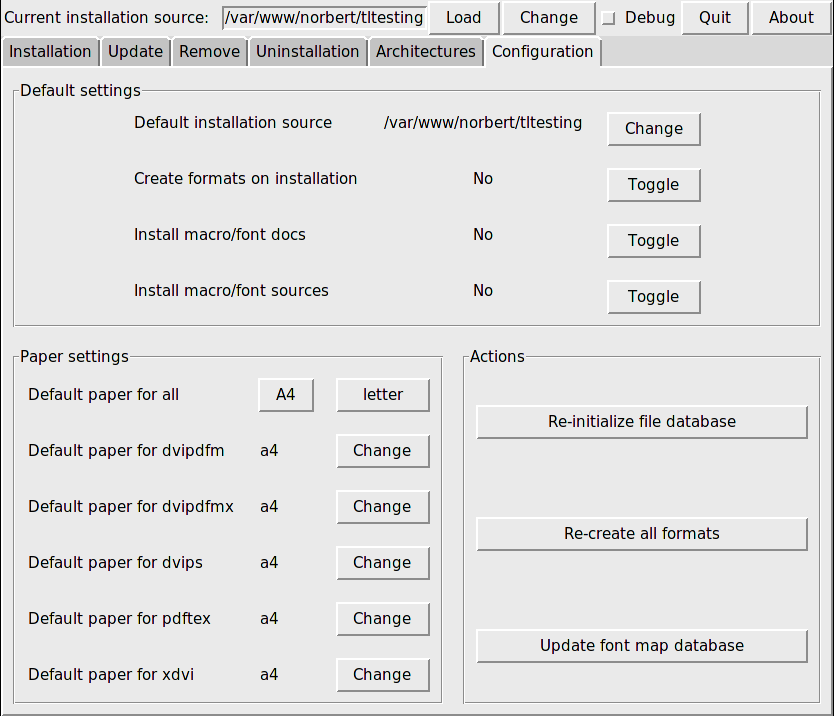
\includegraphics{tlmgrgui-options.png}}
  \caption{\tlmgr\ \acro{GUI} config screen}
  \label{fig:gui:option}
\end{figure}

In the upper part you can change the defaults for the installation
source, whether formats should be created (and updated) by default,
and whether macro/font documentation and source files should be
installed.

In the lower left part you can set the letter for all the programs to
either \texttt{A4} or \texttt{letter}, or for each program
individually. In the latter case you can choose from a wide range of
paper formats depending on the programs support.

In the lower right part there are some convenience buttons for updating
the |ls-R| databases, the outline font list (|updmap-sys|) and
rebuilding all formats.

\subsection{Execution of the commands}

As mentioned above, this \acro{GUI} is only a front end and leaves the
actual work to tlmgr itself. So every action you do (installation,
removal, etc.)\ will pop up a window where the output of the tlmgr
process is shown.

On Unix systems that output will be shown immediately.  Windows
lacks good support for forking in Perl/Tk, and thus you have to wait
until the whole process has terminated before the output appears. That
can take quite some time, so please be patient.

We are working on merging the tlmgr and its \acro{GUI} into one
program so that the output would become more immediate in all cases.


\section{What else is there?}

Besides reworking the whole infrastructure, which is only user-visible in
the new installer and the \tlmgr, as with every year, all the
programs and packages have been updated. We currently ship around~1400
normal packages, e.g., \LaTeX\ and font packages, and
around~300 other packages, mostly documenation and a few packages
which are \tl\ internal. 

The new player in the game
this year is the new engine Lua\TeX\ (\url{http://luatex.org}); besides a
new level of flexibility in typesetting, this provides an excellent
scripting language for use both inside and outside of \TeX\
documents. 


\subsection{Windows-specific features}

To be complete, a \tl\ installation needs support packages that are not
commonly found on a Windows machine. \tl{} provides the missing
pieces:
\begin{description}
\item[Perl and Ghostscript.] Because of the importance of Perl and
  Ghostscript, \tl{} includes `hidden' copies of these
  programs. \tl{} programs that need them know where to find them,
  but they don't betray their presence through environment variables
  or registry settings. They aren't full-scale distributions, and
  shouldn't interfere with any system installations of Perl or
  Ghostscript.
\item[Command-line tools.] A number of Windows ports of common Unix
  command-line programs are installed along with the usual \tl{}
  binaries. These include \cmd{gzip}, \cmd{chktex},
  \cmd{jpeg2ps}, \cmd{unzip}, \cmd{wget} and the
  command-line utilities from the \cmd{xpdf} suite.  (The
  \cmd{xpdf} viewer itself is not available for Windows, but the
  Sumatra \acro{PDF} viewer is based on it:
  \url{http://blog.kowalczyk.info/software/sumatrapdf}.)
\item[\texttt{fc-cache}] helps \XeTeX{} to handle fonts more
  efficiently.
\item[PS\_View.] Also installed is PS\_View, a new PostScript viewer
  that is free software; see fig.~\ref{fig:psview}. It also supports
  viewing of \acro{PDF} files and is extremely fast. Please contact us
  with any suggestions, this program is in active development.
\item[dviout] This is a \acro{DVI} previewer which is shipped only in
  the support directory of the \acro{DVD}, but you will get it if you
  use the network update procedure.  See fig.~\ref{fig:dviout} for a
  screenshot.
\end{description}

\begin{figure}[ht!]
  \centering
  \resizebox{0.8\columnwidth}{!}{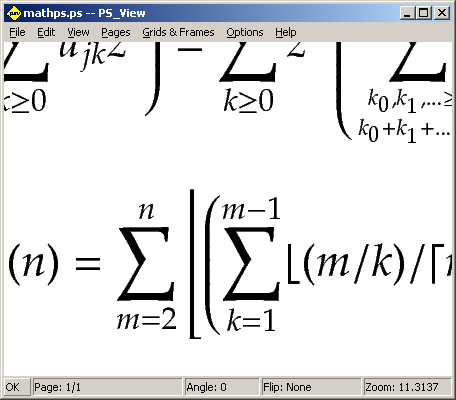
\includegraphics{psview.png}}
  \caption{PS\_View allows very high magnification, and renders
    \acro{PDF}, too}
  \label{fig:psview}
\end{figure}

\begin{figure}[ht!]
  \centering
  \resizebox{0.8\columnwidth}{!}{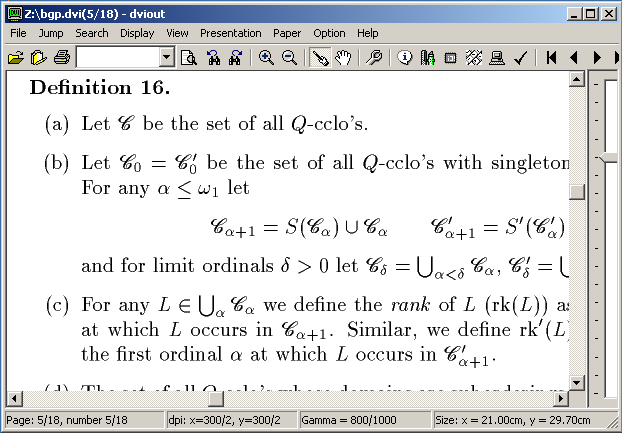
\includegraphics{dviout.png}}
  \caption{DVIout on Windows}
  \label{fig:dviout}
\end{figure}

\section{Final remarks and other resources}

The \tlmgr\ is very much work in progress, and its \acro{GUI} even
more. We are adding new functionality frequently, and improving
existing functionality to make it more robust. If you see any anomalies
don't hesitate to contact us at \url{tex-live@tug.org}, and we
will try to improve it further.

As with most volunteer projects the group of core programmers is
quite small. Most of tlmgr and its \acro{GUI} has been
programmed by the author with some minor contributions from
others. Anyone being more or less able to program Perl is heartily
invited to join forces and help us, there are long lists of
\acro{TODO}s for the \tlmgr, let alone for all of \tl.

If you are searching more information on \tl\ your first starting
place should be \url{http://tug.org/texlive/} and the documentation
specific page \url{http://tug.org/texlive/doc.html}.

The list of people to thank is too long to be included here, please
see the online \tl\ documentation, Chapter~9
(Acknowledgments), for the ever growing list. Of course one name has to
be mentioned and that is Karl Berry who with great enthusiasm and
perpetual support (and a sometimes critical voice if I was too fast in
implementing something!)\ prepared the \tl~2008 release.

\bibliographystyle{arstexnica}
\bibliography{tlmgr-article}

%
% END OF ARTICLE
%
\end{article}
\end{document}


